\section{Conclusion}

Dans cette partie, nous avons étudié les concepts fondamentaux de RADOS, la solution de stockage distribuée centrale de Ceph. Nous avons vu que l'un de ses enjeux centraux est d'éliminer les points de failles uniques pouvant mettre en péril l'infrastructure. 

Pour ce faire, chaque nœud du cluster de stockage prend en charge une partie de l'intelligence et de la complexité du système, à l'aide d'une version locale de l'état du cluster. Cette version est mise à jour à mesure que les composants interagissent entre eux. Le placement des données est géré par un algorithme baptisé CRUSH. 

De plus, pour garantir des performances optimales, RADOS utilise un système de stockage d'objets tout en introduisant un panel de structures logiques facilitant la manipulation des données. Enfin, certains sites sont responsables de groupes d'objet et doivent assurer leur cohérence et leur pérennité au sein du cluster. 

La figure \ref{chap2:dataFlow} se propose de synthétiser l'ensemble des notions abordées dans cette partie. Elle illustre une première demande de stockage d'objets effectuée par un utilisateur de RADOS.

\hspace*{-2in}
\begin{figure}[h]
    \centering
    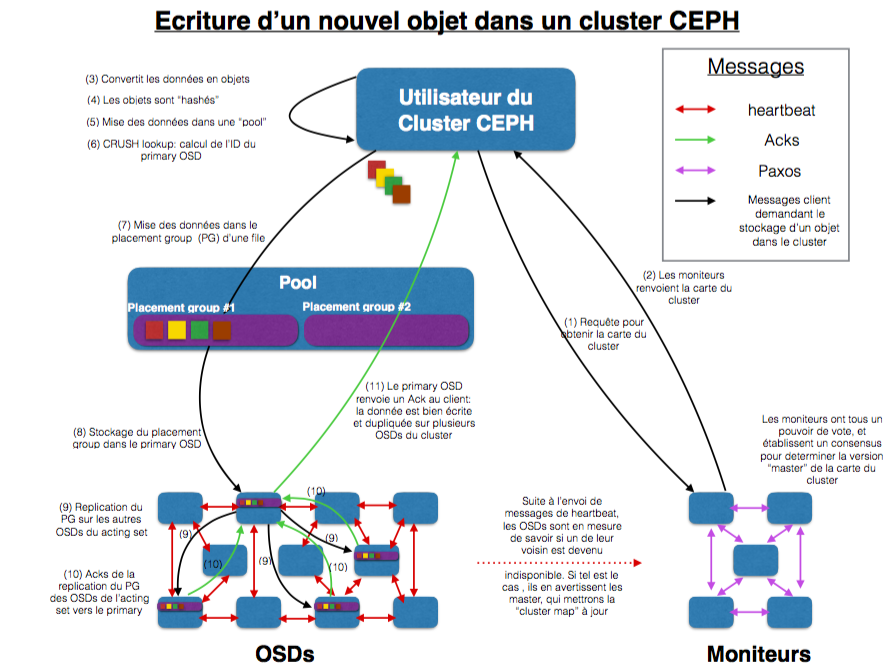
\includegraphics[scale=.5]{./images/dataFlow.png}
    \caption{Aperçu des différentes actions entreprise par les composants du cluster lorsqu'un utilisateur désire stocker une donnée dans le cluster.	}
    \label{chap2:dataFlow}
\end{figure}